\section{Durchführung}

Das verwendete Verfahren spiegelt ein Shadow Volumes artiges Verfahren im zweidimensionalen Raum wieder. Auch hier wird die Silhouette des angestrahlten Rechtecks berechnet und and die Grenzen, des Fensters auf dem Bildschirm, projiziert. Der von dieser Projektion abgedeckte Bereich wird dunkler eingefärbt.

Der Rasterizer, welche die Schattenfläche auf die Lichtwerte der Pixel in dem Fenster anwendet, benötigt zwei Strahlen, welche die Projektion der Silhouette darstellen, und ein Array von Punkten welche alle Eckpunkte des Rechtecks, welche auf der dunklen Seite des Objektes liegen, enthält. Diese werden benötigt, damit der Schatten das Rechteck nicht teilweise bis ganz überdeckt. Somit kann man die Objekte in der Szene besser voneinander unterscheiden und sieht nicht ausschließlich schwarze Flächen.

Es wird vor jeder Berechnung der Schatten von einem vollkommen beleuchteten Raum ausgegangen. Dazu wird für jeden Pixel auf dem Bildschirm der Wert 1, von allen Lichtquellen beleuchtet, gespeichert.

%\begin{figure}[t]
%	\centering
%	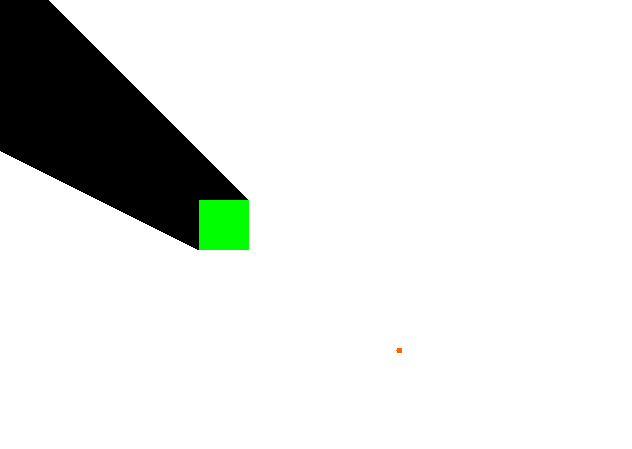
\includegraphics[width=\columnwidth]{images/durchfuehrung.png}
%	\caption{einfacher Schatten}
%	\label{fig:durch1}
%\end{figure}

Im Folgenden wird die entwickelte Methode gezeigt um einen Schatten zu berechnen, wie er zum Beispiel in Abbildung \ref{fig:durch1} zu sehen ist.

%\begin{figure}[t]
%	\centering
%	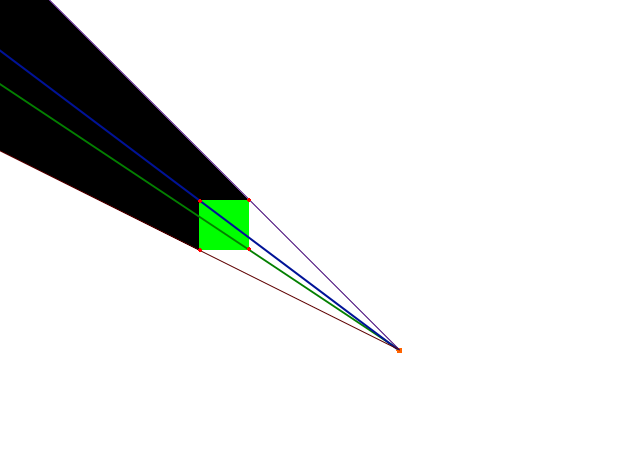
\includegraphics[width=\columnwidth]{images/durchfuehrung_1.png}
%	\caption{Geraden durch Eckpunkte}
%	\label{fig:durch2}
%\end{figure}

Im ersten Schritt der Berechnung werden durch jeden Eckpunkt
\begin{equation}
	P = \left(\begin{array}{c} p_1 \\ p_2 \end{array}\right)
\end{equation}
des schattenwerfenden Objektes und die Lichtquelle
\begin{equation}
	L = \left(\begin{array}{c} l_1 \\ l_2 \end{array}\right)
\end{equation}
Geraden
\begin{equation}
	\vec{g} = \left(\begin{array}{c} p_1 \\ p_2 \end{array}\right) + r * \left(\begin{array}{c} p_1 - l_1 \\ p_2 - l_2 \end{array}\right)
\end{equation}
gelegt (Abbildung \ref{fig:durch2}).

%\begin{figure}[t]
%	\centering
%	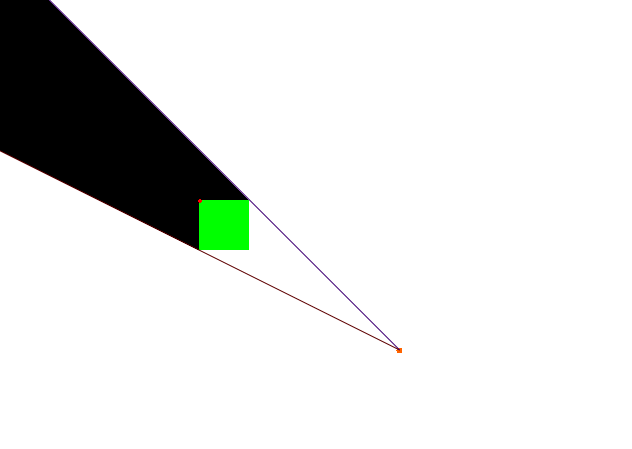
\includegraphics[width=\columnwidth]{images/durchfuehrung_4.png}
%	\caption{Geraden mit größtem Winkel}
%	\label{fig:durch3}
%\end{figure}

%\vec{e}_1=\left(\begin{array}{c} 1 \\ 0 \end{array}\right)

Ausschlaggebend für den geworfenen Schatten sind die zwei Geraden, deren Winkel am weitesten auseinander liegt (Abbildung \ref{fig:durch3}). Dazu wird rekursiv jedes Geradenpaar

\begin{equation}
	\vec{g}_1 = \vec{o}_1 + r * \vec{m}_1, \vec{g}_2 = \vec{o}_2 + s * \vec{m}_1
\end{equation}
durch den Winkel
\begin{equation}
	\omega = arccos(\vec{m}_1 * \vec{m}_2 / (|\vec{m}_1| * |\vec{m}_2|))
\end{equation}

mit dem vorherig größten Geradenpaar verglichen und das mit dem größeren Winkel zurückgegeben.

%\begin{figure}[t]
%	\centering
%	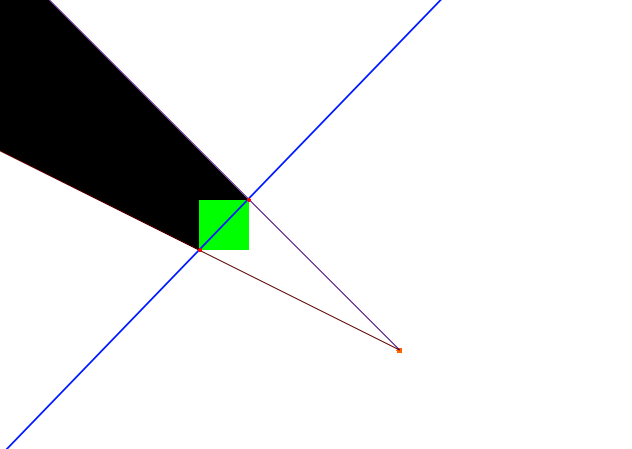
\includegraphics[width=\columnwidth]{images/durchfuehrung_2.png}
%	\caption{Gerade durch Ortsvektoren}
%	\label{fig:durch4}
%\end{figure}

Damit später die Objekte nicht vom eigenen Schatten teilweise bis ganz überdeckt werden, werden nun die Eckpunkte des Rechtecks berechnet, welche auf der dunklen Seite des Objektes liegen. Dazu wird eine Gerade durch die Ortsvektoren der zwei vorher bestimmten Geraden bestimmt (Abbildung \ref{fig:durch4}).

\begin{equation}
	s: \vec{s} = \vec{o}_1 + t * \left(\begin{array}{c} o_21 - o_11 \\ o_22 - o_12 \end{array}\right)
\end{equation}

%\begin{figure}[t]
%	\centering
%	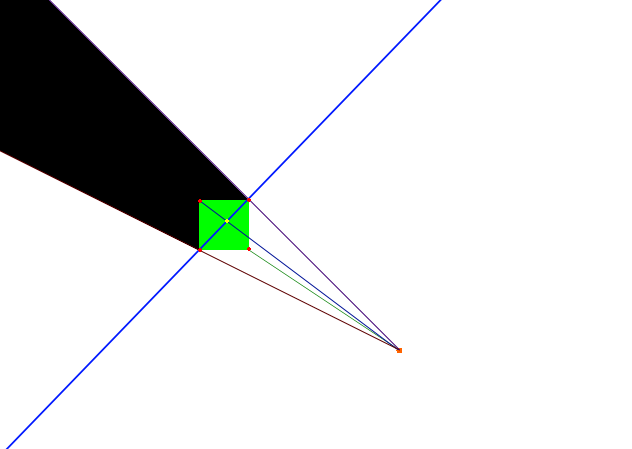
\includegraphics[width=\columnwidth]{images/durchfuehrung_3.png}
%	\caption{Eckpunkte auf der dunklen Seite}
%	\label{fig:durch5}
%\end{figure}

Wenn ein Schnittpunkt zwischen der Geraden $s$ und der Strecke zwischen einem Eckpunkt des Rechtecks und der Position der Lichtquelle vorhanden ist hängen wir diesen Eckpunkt an das an den Rasterizer zu übergebende Array an (Abbildung \ref{fig:durch5}).
